\chapter{TypeScript}
Para convertir un archivo ts a js en un power shell de windows en modo administrador ejecutamos el siguiente comando.\\
\textbf{Set-ExecutionPolicy RemoteSigned}
\begin{figure}[H] 
	\centering
	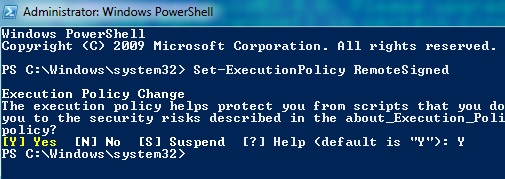
\includegraphics[scale=1]{images/c2_1.jpg}
	\caption{Configurando TypeScript.}
\end{figure}

Ejecutamos el siguiente comando para obtener el js:\\
\textbf{tsc archivo.ts}\\

\begin{figure}[H] 
	\centering
	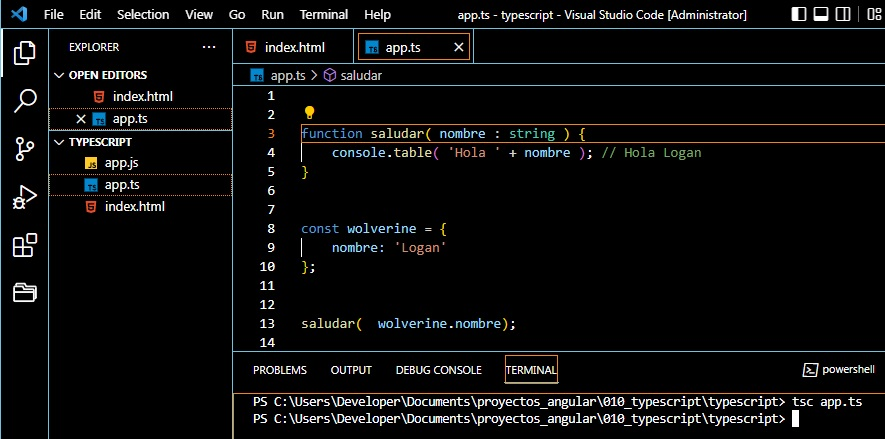
\includegraphics[scale=0.65]{images/c2_2.jpg}
	\caption{Convirtiendo ts a  js.}
\end{figure}

Ejecutamos el siguiente comando para obtener el archivo de configuracion de TypeScript :\\
\textbf{tsc --init}\\

Ejecutamos el siguiente comando para que TypeScript quede en modo de observador, para que traduzca al detectar un cambio:\\
\textbf{tsc -w}\\


\section{Let y var}
Let: Existe solo entre las llaves de cierre que se encuentre,solo en ese ambito y se queda con el tipo de dato que se inicio. Reserva otro espacio en memor\'\i{}a al ser declarada.\\
Var: Redefine el mismo espacio en memor\'\i{}a .
\begin{figure}[H] 
	\centering
	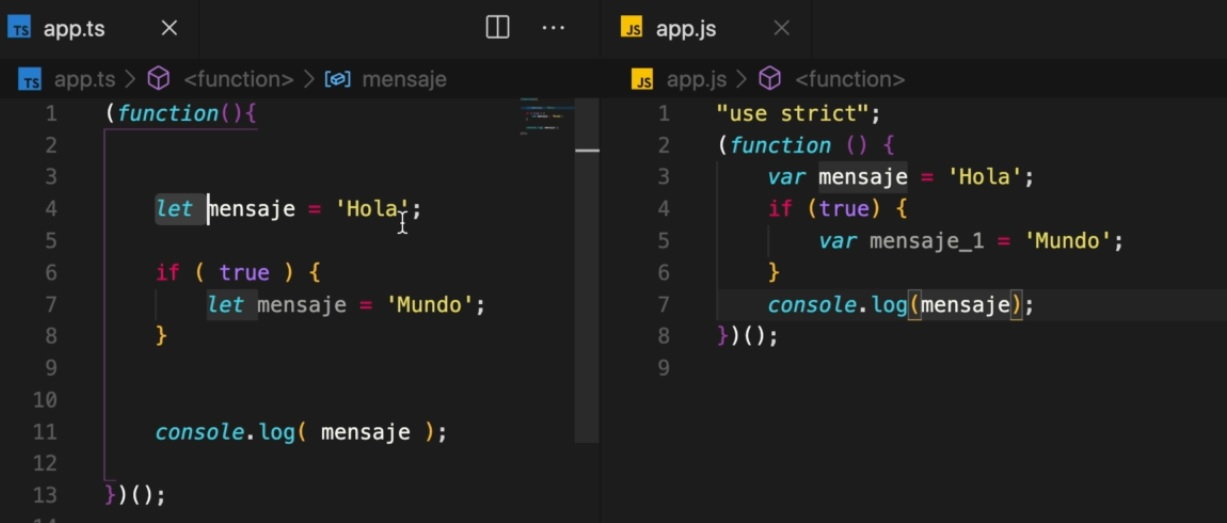
\includegraphics[scale=0.45]{images/c2_3.jpg}
	\caption{Let reserva otro espacio en memor\'\i{}a.}
\end{figure}

\section{Tipos de datos.}
\begin{figure}[H] 
	\centering
	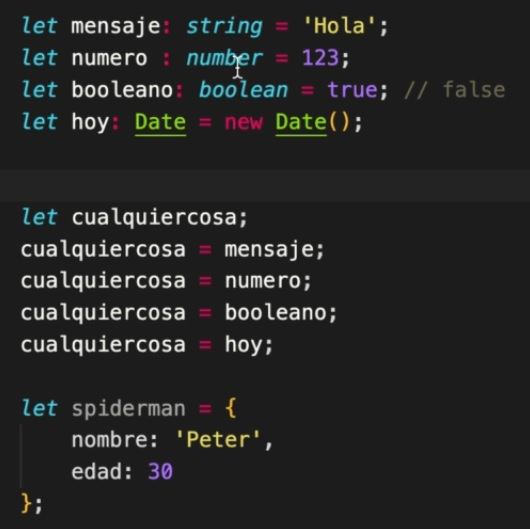
\includegraphics[scale=0.6]{images/c2_4.jpg}
	\caption{Tipos de datos.}
\end{figure}

\section{Template literales.}
\begin{figure}[H] 
	\centering
	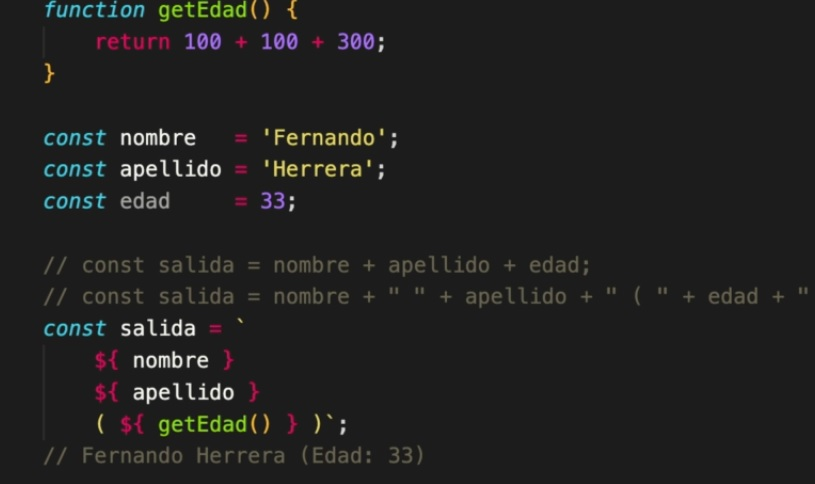
\includegraphics[scale=0.6]{images/c2_5.jpg}
	\caption{Template literales.}
\end{figure}

\section{Promesas.}
\begin{figure}[H] 
	\centering
	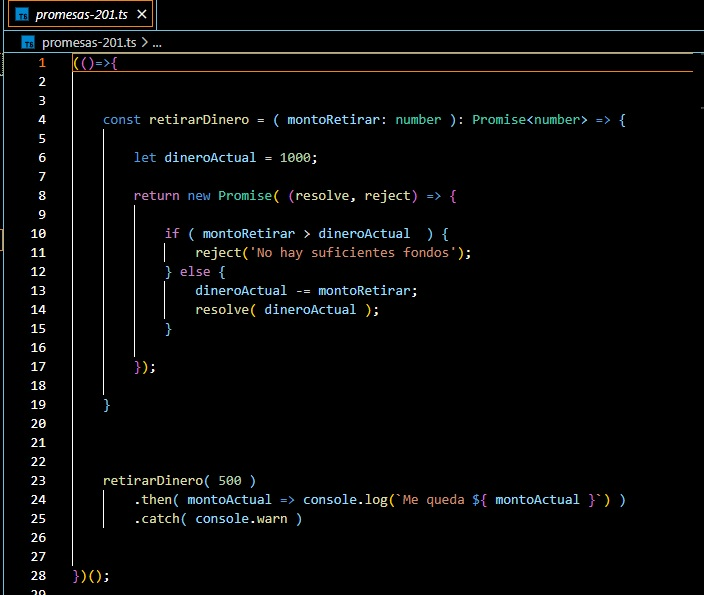
\includegraphics[scale=0.8]{images/c2_5_1.jpg}
	\caption{Promesas.}
	
\end{figure}

\section{Interfaces.}
Sirve para definir reglas.
\begin{figure}[H] 
	\centering
	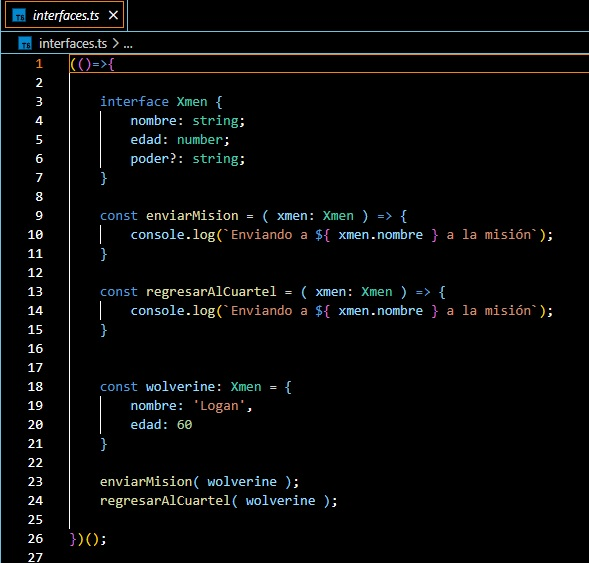
\includegraphics[scale=0.8]{images/c2_6.jpg}
	\caption{Interfaces.}
\end{figure}

\section{Importaciones.}
Para importar un proyecto abrimos la carpeta con Visual Studio Code y ejecutamos
en la terminal.Para instalar las dependencias\\
\texttt{npm install}\\
Para iniciar el proyecto.\\
\texttt{npm start}\\




